\section{Nao SDK}

In diesem Abschnitt wird das \ac{SDK} des Nao Roboters vorgestellt. Dazu gehört die Erläuterung des \textit{NAOqi Frameworks}, dem \textit{.NET SDK} und der eigentlichen Programmierung.

\subsection{NAOqi Framework}
NAOqi ist der Name der Software die tatsächlich auf dem Roboter läuft und ihn kontrolliert. Das NAOqi Framework ist das Gerüst um Nao zu programmieren. Es spricht auf die gewöhnlichen Anforderungen in der Robotertechnik an: Parallelität (von Threads), Ressourcen, Synchronisation und Events. Das bedeutet, es kann mit allen gängigen Techniken der Software - Entwicklung bedient werden. 

Dieses Framework erlaubt homogene Kommunikation zwischen verschiedenen Modulen (Bewegung, Autio, Video), homogene Programmierung und homogenes Teilen von Informationen über die verschiedenen Module hinweg.
\\
\\
\noindent
Das NAOqi - Framework beinhaltet folgende Gesichtspunkte:
\begin{itemize}
\item Cross - Plattform
\item Cross - Language
\item NAOqi - Prozess
\item Module
\end{itemize}

\noindent
\textbf{Cross - Plattform}
\\
Cross - Plattform bedeutet Plattformunabhängigkeit gegenüber dem Betriebssystem auf dem Programmiert werden soll. Sowohl auf Linux, Windows und auf Mac kann Code für Nao programmiert werden. Allerdings kann auf Windows und Mac nur Code auf dem Computer selbst kompiliert werden, während auf Linux der Code auch auf dem Roboter selbst programmiert werden kann.
\\
\\
\textbf{Cross - Language}
\\	
Cross - Language ist nach \cite{ws:naodocu} die Eigenschaft, dass Software in C++ und in Python entwickelt werden kann. In allen Fällen, in denen die Methoden exakt gleich sind kann die \ac{API} (dt: Programmierschnittstelle), gleichgültig von welcher der unterstützten Programmiersprachen, aufgerufen werden. Die \ac{API} ist in acht Programmiersprachen verfügbar: C++, Python, .NET (C\#, Visual Basic, F\#), Java, Matlab und Urbi.

Neue NAOqi Module können nur in C++ oder Python entwickelt werden, jedoch kann die Client - API mit allen Programmiersprachen angesprochen werden. Ebenso sind nur C++ und Python auf dem Roboter unterstützt, die anderen Sprachen werden nur über \textit{Remote - Access} unterstützt. (siehe unten \textit{Proxy})
\\
\\
\textbf{NAOqi - Prozess}
\\
Der NAOqi - Prozess der auf dem Roboter läuft ist ein \textit{Broker} (siehe unten). Beim Start des Prozesses wird eine Konfigurationsdatei \textsf{autoload.ini} geladen, die definiert, welche Bibliotheken geladen werden sollen. Jede Bibliothek beinhaltet ein oder mehrere Module, die der Broker nutzt um deren Methoden öffentlich anzuzeigen. (siehe \ref{f:naoqi_broker1})

\begin{figure}[H]						
	\centering							
	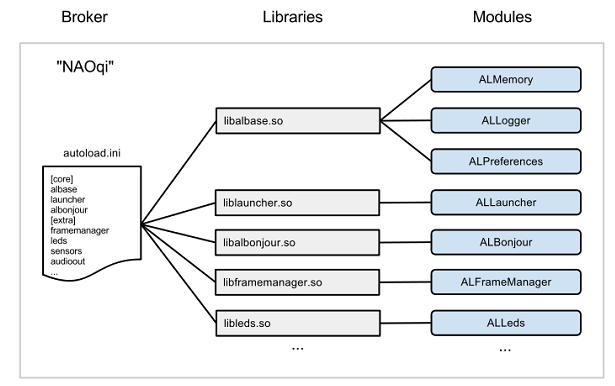
\includegraphics[scale=0.8]{Bilder/naoqi_process1.PNG}
	\caption{NAOqi Broker}						
	\label{f:naoqi_broker1}						
\end{figure}

Der Broker 	stellt einen Lookup - Service zu Verfügung, so dass jedes Modul im Baum oder verteilt im Netzwerk jede Methode finden kann, die öffentlich angezeigt wurde.

Das Laden der Module zum Start erzeugt einen Baum von Methoden, die an Module geknüpft und diese wiederum an einen Broker geknüpft sind. (siehe \ref{f:naoqi_broker2})

\begin{figure}[H]						
	\centering							
	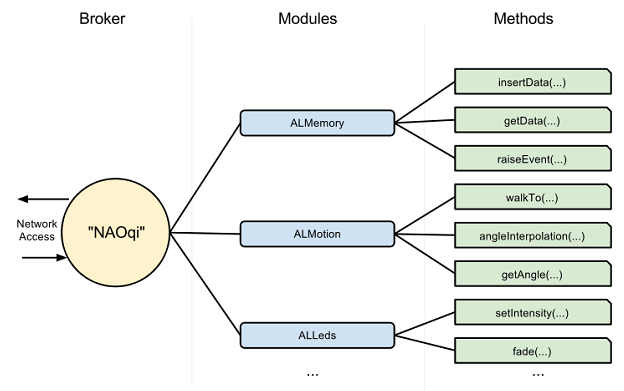
\includegraphics[scale=0.8]{Bilder/naoqi_process2.PNG}
	\caption{NAOqi Method-Tree}						
	\label{f:naoqi_broker2}						
\end{figure}
\noindent
\textbf{Broker}
\\
Der Broker ist ein Objekt, der zwei generelle Rollen einnimmt. Erstens ist das ein Verzeichnis - Dienst, mit dessen Hilfe Module und Methoden gefunden werden können und zweitens ein Netzwerk - Anschluss, der es möglich macht Methoden verknüpfter Module auch außerhalb des Prozesses aufzurufen.

Die Meiste Zeit muss sich keine Gedanken um die Broker gemacht werden, da diese ihre Arbeit selbstständig und transparent machen. Geschriebener Code kann gleich sein, ob für Aufrufe an "`lokalen Module"' (gleicher Prozess) oder "`entfernte Module"' (anderer Prozess oder anderes System).
\\
\\
\textbf{Proxy}
\\
Ein Proxy ist ein Stellvertreter - Objekt das sich genau so verhält, wie das Modul das es repräsentiert. Wenn ein Proxy - Objekt des ALMotion Moduls instanziiert wird, erhält das Proxy - Objekt auch alle Methoden des ALMotion Moduls.

Um ein Proxy eines Moduls zu instanziieren gibt es zwei Möglichkeiten: 
\begin{itemize}
\item Nur den Namen des Moduls benutzen. In diesem Fall muss der auszuführende Code und das Modul das verbunden werden soll im selben Broker liegen. Dies ist ein "`lokaler"' Aufruf
\item Zusätzlich zum Namen des Moduls auch die IP und den Port des Broker benutzen. In diesem Fall muss das Modul im zugehörigen Broker liegen. Dies ist ein "`entfernter"' Aufruf.
\end{itemize}
Der genaue Unterschied zwischen lokalen und entfernten Modulen wird im folgenden erklärt.
\\
\\
\textbf{Module}
\\


\subsection{.NET SDK}

Naoqi (architektur, modell)
	embedded
	
choreographe \& naoqi	


verfügbare sprachen


vorstellung c\#